% For a masters thesis, replace the above \documentclass line with
% \documentclass[masters]{ucbthesis}
% This affects the title and approval pages, which by default calls this
% document a "dissertation", not a "thesis".

\documentclass[masters]{ucbthesis}

% support display of graphics
\usepackage{graphicx}

% import library of technical symbols
\usepackage{amsmath,amssymb,latexsym}

% import bibliography tools
\usepackage{natbib}
\citestyle{aa}

% To compile this file, run "latex thesis", then "biber thesis"
% (or "bibtex thesis", if the output from latex asks for that instead),
% and then "latex thesis" (without the quotes in each case).

% Double spacing, if you want it.  Do not use for the final copy.
% \def\dsp{\def\baselinestretch{2.0}\large\normalsize}
% \dsp

% If the Grad. Division insists that the first paragraph of a section
% be indented (like the others), then include this line:
% \usepackage{indentfirst}

\begin{document}

% Declarations for Front Matter

\title{HYPERION: The Case for Interferometry in 21 cm Reionization Global 
Signal Studies}
\author{Kara Kundert}
\degreesemester{Fall}
\degreeyear{2018}
\degree{Master of Astrophysics}
\chair{Professor Aaron Parsons}
\othermembers{Professor Martin White \\
  Professor Eugene Chiang}
\numberofmembers{3}
\field{Astronomy}
\campus{Berkeley}

\maketitle
% Delete (or comment out) the \approvalpage line for the final version.
\approvalpage
\copyrightpage

% (This file is included by thesis.tex; you do not latex it by itself.)

\begin{abstract}

% The text of the abstract goes here.  If you need to use a \section
% command you will need to use \section*, \subsection*, etc. so that
% you don't get any numbering.  You probably won't be using any of
% these commands in the abstract anyway.

We seek to examine the case for the viability of using a classical 
 interferometer to search for the ``global signal" of 21 cm emission from 
 reionization. In particular, we examine how spatial windowing can be used to 
 redistribute a spatial monopole into higher order modes that are accessible to 
 the interferometer. In this study, the windowing is managed through the use of 
 absorptive walls around the individual antennas of the array, which modify 
 each antenna's receptivity of the sky, thus introducing spatial variation into 
 the monopole signal. We can characterize the parameters of these walls and 
 their effects on our observed signal into a set of known sensitivity 
 coefficients, which can then be used to accurately recover the reionization 
 global signal. Preliminary results show that this method does have some 
 sensitivity to the monopole, indicating that it could serve as an alternative 
 experimental design to the traditional single-dish approach, as it benefits 
 from different systematics and finer control of spatial scaling and 
 sensitivity, which may help to mitigate non-isotropic foregrounds.

\end{abstract}


\begin{frontmatter}

\begin{dedication}
\null\vfil
\begin{center}
 \noindent{\large{\emph{Failure is simply the opportunity to begin again,\\ 
 this time more intelligently.}}\\ \normalsize{-- Henry Ford}}
\end{center}
\vfil\null
\end{dedication}

% You can delete the \clearpage lines if you don't want these to start on
% separate pages.

\tableofcontents
\clearpage
\listoffigures
\clearpage
%\listoftables

\begin{acknowledgements}
 This work would not have been possible without the financial support of the 
 National Science Foundation CAREER Award, the International House Carl \& 
 Betty Helmholz Gateway Fellowship, or the University of California, Berkeley 
 Department of Astronomy. 

 I must also give ample thanks to those with whom I have had the pleasure of 
 working on this and related projects. In particular, I would like to thank 
 Cherie Day, who has given me her love, her support, and her valuable 
 scientific and engineering insights since my first day on the Berkeley campus.  
 I would also like to thank the past and present members of the HYPERION team, 
 including Nipanjana Patra, Sanah Bhimani, Trisha Bhattacharya, Daniel Shen, 
 Raj Biswas, and Liju Phillip. Their hard work, patience, and, at times, upper 
 body strength, have made this project what it is today.  I could not have 
 reached this point without their combined abilities, and I am endlessly 
 grateful for their contributions.

 I would also like to thank the various members of the department who have 
 helped me along the path to completing this thesis. To Fatima Abdurrahman, 
 thank you for the dumplings and your friendship. To Charles Goullaud, thank 
 you for letting me unload my stress over some of your very fine whiskey and 
 some very silly movies. To Deepthi Gorthi, thank you for walking with me when 
 I needed to get out of the department and get some perspective. To Tom Zick, 
 Carina Cheng, and Zaki Ali, thank you for stepping in and providing me with 
 support when I most needed it.

 I am so grateful to my friends outside of the department, who have been 
 endlessly and creatively supportive along this journey. To Tristan Scroggins, 
 thank you for believing in me when I did not. To Tj Carskadon, thank you for 
 always being there for me, no matter whether I need career advice, a study 
 buddy, a drinking partner, a pep talk, or a hug.  To Cameron Chalker, thank 
 you for not listening to my excuses and always driving me to give my best, and 
 for reminding me of the consequences of reneging on our long-standing deal.

 Finally, I cannot adequately express how grateful I am to my father. He has 
 always been my greatest ally and continues to support me in every way he can. 
 I would not have been able to complete this thesis without him standing 
 steadfastly in my corner.

\end{acknowledgements}

\end{frontmatter}

\pagestyle{headings}

\chapter{The Global Signal -- Its Physics and Significance to Cosmology}

\section{Overview of the Epoch of Reionization}

In brief, the Epoch of Reionization refers to the period of the universe's 
history during which its supply of intergalactic hydrogen became reionized.  
This is important to its evolution, and therefore of interest to astronomers, 
due to the driving factor of that ionization: the ignition of the first stars, 
galaxies, and black holes in the universe. A positive detection of the Epoch of 
Reionization will help astronomers to clarify many open questions of cosmology, 
such as the properties of the first galaxies, how stars with zero metallicity 
formed, the physics of early quasars, and more.

In slightly more detail, let us begin at the beginning. At the start of time, 
the universe was extremely hot and ionized from the Big Bang. Over time, as 
space itself expanded and the gas within the universe cooled adiabatically 
along with that expansion, the temperature of the universe dropped low enough 
that the nearly uniform ionized plasma that made up the universe was able to 
recombine to form neutral hydrogen. This phase transition, which occurred 
approximately 400,000 years after the Big Bang, enabled photons to decouple 
from the baryonic matter, allowing photons to stream freely for the first time 
in the history of the universe.  Those photons are what we now know as the 
``Cosmic Microwave Background" (CMB).

At the point of the CMB, the gravitational force had heretofore always served 
as second fiddle to the electromagnetic force, and the formation of structure 
was driven solely by dark matter~\citep{zaroubi2012}.  As such, structure had 
yet to form, and the release of the CMB led to a period known as the ``Dark 
Ages" -- a time when the universe had nothing to do but slowly get to work 
allowing slight matter over-densities to grow and transform into stars, 
galaxies, and black holes.

So, about 100 million years passed and the universe bathed in nothing but the 
after-glow of the Big Bang. Finally, the first galaxies formed, and along with 
them bright stars to emit ionizing radiation. Soon, we find small ionized 
bubbles in the intergalactic medium (IGM), the hydrogen gas filling the space 
between galaxies. Over time, more galaxies and their bright stars make more 
ionized bubbles, until eventually the entire universe's supply of loose 
hydrogen gas has been converted into a proton-electron ionized plasma.

This period, very creatively, is called the Epoch of Reionization -- the epoch 
during which the universe once again became ionized, like it was at the dawn of 
time.

As of yet, there has been no confirmed\footnote{While there has yet to be a 
confirmed direct detection of the Epoch of Reionization, the EDGES experiment 
has announced a possible detection of the 21 cm reionization global 
signal~\citep{bowman2018}.} direct detection of this time period -- either of 
the objects that drive it nor of the gas behavior itself.  This is not for lack 
of trying.  There are currently (or soon to be) observatories looking for 
high-redshift galaxies and quasars~\citep{gardner2006}, for power-spectrum 
measurements to find ionized regions around those high-energy 
objects~\citep{deboer2017}, and for the microscopic temperature changes in the 
gas of the universe~\citep{bowman2010}.  As it turns out, these observations 
are hard to make -- 13 billion light years is a long way for light to travel.

For the sake of brevity and intellectual focus, this thesis (and the experiment 
proposed within) will be focusing solely on observing the overall average 
behavior of the intergalactic medium as it evolves throughout this time period.  
This is referred to as the ``global signal".

\section{Overview of the Global Signal}

The global signal of reionization is an observation of the overall average 
nature of hydrogen throughout this epoch, i.e. the spatially averaged signal 
from the neutral hydrogen gas, as observed using redshifted 21 cm emission from 
the intergalactic medium 13 billion years ago. More specifically, global signal 
experiments seek to observe the relationship between the gas temperature and 
the ambient temperature of the universe, as set by the CMB photons.  By 
observing the evolution of the thermal gas temperature ($T_K$) relative to the 
photon temperature ($T_\gamma$), we are able to better understand how and when 
energy was injected into the gas~\citep{pritchard-loeb2010}. For example, the 
X-rays generated by black holes contributed to the heating of the gas, making 
the gas itself brighter than the ambient photons. Additionally, Lyman-$\alpha$ 
photons from Population II and III stars modify the coupling of the IGM gas 
temperature to the 21 cm spin temperature via the Wouthuysen-Field effect, 
providing a means to track early star formation~\citep{furlanetto2006}.

This signal ($T_b$) is measured as a function of four main variables -- the 
thermal temperature of the hydrogen gas ($T_K$), the volume-averaged ionized 
fraction of hydrogen ($x_i$), the specific flux of the Lyman-$\alpha$ frequency 
($J_\alpha$), and the number density of hydrogen ($n_H$). There are six main 
physical regimes believed to have taken place during the process of structure 
formation and IGM reioization, which can be seen in 
Fig.~\ref{fig:global-signal} and are physically detailed below.

\begin{figure}
    \begin{center}
    \includegraphics[width=\linewidth]{global_signal.png}
    \end{center}
    \caption{
        In the top half of the figure, we see a cartoon of the reionization 
        history of the universe and the development and growth of ionized 
        bubbles over time. In the bottom half, we see a breakdown of $T_b$, the 
        brightness temperature of the 21 cm global signal, over time. There are 
        five labeled regimes to this plot, each corresponding to the dominance 
        of a different variable in the production of the 21 cm signal. Figure 
        originally published in~\citealp{pritchard-loeb2012}.
    }
    \label{fig:global-signal}
\end{figure}

\subsection{Brief History of the Global Signal}
\begin{itemize}
    \item[--] (200 $\leq z \leq$ 1100): During this time period, the residual 
     free electron fraction remaining post-recombination and the high gas 
     density allows the thermal and spin temperatures of the gas to remain 
     coupled with the photon background via Compton scatting and collisional 
     excitations. All temperatures are the same, and therefore there will be no 
     detectable 21 cm signal.
    \item[--] (40 $\leq z \leq$ 200): As cosmological expansion continues, 
     Compton scattering no longer couples the thermal temperature of the gas to 
     the CMB photons, and the gas and radiation decouple and go out of 
     equilibrium.  Collisional coupling sets the spin temperature $T_S < 
     T_\gamma$, leading to an absorption feature in the 21 cm global signal.  
    \item[--] (30 $\leq z \leq$ 40): Expansion continues and collisional 
     interactions are no longer effective at coupling the thermal and spin 
     temperatures of the gas. The excitation levels shift to being set by 
     radiative coupling to the CMB, such that $T_S = T_\gamma$, and there is no 
     detectable 21 cm signal.
    \item[--] (15 $\leq z \leq$ 30): As the first sources (e.g. stars, active 
     galactic nuclei (AGN), etc...) ignite, they begin emitting high energy 
     Lyman-$\alpha$ and X-ray photons. The hyperfine populations couple to the 
     thermal temperature of the cold gas via the Wouthuysen-Field effect, such 
     that $T_S \sim T_K < T_\gamma$, resulting in an absorption feature in the 
     21 cm global signal.
    \item[--] (7 $\leq z \leq$ 15): The radiation (particularly the X-rays) 
     from bright sources heat the gas, $T_K > T_\gamma$ and we see 21 cm 
     emission in the global signal. Lyman-$\alpha$ coupling is still effective 
     at setting the level populations.
    \item[--] ($z \leq$ 7): Enough ionizing radiation has spread throughout the 
     universe that the IGM has been converted from neutral to ionized, and 
     reionization is complete.
\end{itemize}

At present, all redshift ranges listed are theoretical, as no confirmed 
detections have yet been made. However, it is abundantly clear that detection 
and study of this era of this part of the universe's history is rich with 
information about our cosmological origins, and could fill many of the gaps in 
our current knowledge.

\chapter{Interferometry}

\section{Brief Overview}
\label{sec:brief-overview}

Let's start with what they are. An interferometer is any device which 
superimposes the waves from a coherent light source in order to gain 
information about the source itself. So what does that mean? Let's look at the 
most basic case of a Michelson interferometer. In this scenario, we have a 
coherent light source (typically a laser) pointing at a beam splitter. The 
splitter splits the light into two identical beams, which travel on separate 
paths, until they are recombined before entering a detector. The difference in 
the paths creates a phase difference between the beams. This phase difference 
is what creates an interference pattern, which is what then gives us the 
information we seek about the light source, which typically comes in the form 
of fringes. 

What if instead of using mirrors and beam splitters, we built two identical 
small telescopes that were physically separated in space, then pointed them at 
the same astronomical source. Because they're not in the same spot but are 
separated by a ``baseline", there must be a difference in the path lengths 
between the telescopes and the source. This is the fundamental idea behind 
radio interferometers. Now let's explore the mathematics.

In order to get a handle on the mathematics and theory behind astronomical 
interferometry, we're going to make some simplifying assumptions. We will 
consider the case of a two-element interferometer (that is, an interferometer 
with two antennas and one ``baseline" between them) observing a very distant 
source (so the emissions from the source will come in the form of plane waves 
and the antennas will point in the same direction on the sky).  This 
interferometer will be fixed in space - so, no rotation or motion of the 
antennas themselves.  We will also be looking at just one frequency, so the 
signals coming in will be perfectly sinusoidal with one known wavelength.  We 
won't be worrying about anything in the backend, so we'll say that we have no 
frequency conversions (an RF interferometer) with a single polarization and 
perfectly idealized electronics (perfectly linear, no amplitude or phase 
distortions, perfectly identical for both instruments, and no added noise).  
We'll also assume no propagation distortions, so the plane waves we observe 
from the source won't be disturbed by the ionosphere or atmosphere of Earth, 
and that the source is small enough in angular size that we can approximate the 
sky as flat and two-dimensional. 

What does that leave us? Two identical sensors that are separated by a vector 
distance $\mathbf{b}$ - this is our baseline. These sensors are both pointed at 
a quasi-monochromatic source of frequency $\nu$, in the vector direction 
$\mathbf{s}$.  Combining these fundamental numbers, we then get the key 
quantity $\tau_g = \mathbf{b} \cdot \mathbf{s} / c$, which is the geometric 
time delay. That's the extra time needed for the signal to reach the more 
distant antenna. This number will be important to us in order to correlate our 
signals.  We can also find the phase shift in the signal by writing $\Theta = 
\omega \tau_g = 2 \pi \mathbf{b} \cdot \mathbf{s} / \lambda$.

With this knowledge of the phase difference between the paths, we can write out 
the voltages received by each of the sensors, so we get $V_1 = E \cos{[\omega(t 
- \tau_g)]}$, because it has that extra phase delay from the baseline 
separation, and $V_2 = \cos{(\omega t)}$. In this case, the path lengths from 
the sensor to the multiplier are treated as being equal, so we don't need to 
add any extra phase terms. We then multiply our signals together, and take an 
average over time, which gives us an averaged product $R_C = P \cos{(\omega 
\tau_g)}$. This quantity is dependent on the received power $P = E^2/2$ and the 
geometric delay $\tau_g$, and hence on the baseline orientation and source 
direction. We can rewrite $R_C$ to make this relationship more explicit as:

\begin{equation}
    R_C = P \cos{(2 \pi \frac{\mathbf{b} \cdot \mathbf{s}}{\lambda})}
    \label{eq:R_C}
\end{equation}

Note that $R_C$ is not a function of the time of the observation (so long as 
the source itself is not transient or variable), the physical location of the 
baseline (provided that the source is in the far field, which is always true of 
astronomical sources), or the actual phase of the incoming signals.  All that 
matters is the relative phase between the sensors!

In order to get a better understanding of our observed response, let's rewrite 
some terms. Let us say that $\mathbf{b} \cdot \mathbf{s}/\lambda = 
u\cos{\alpha} = u\sin{\theta} = ul$. In this case, we are defining 

\begin{equation}
    u \equiv b/\lambda
    \label{eq:u}
\end{equation}

\noindent which is the baseline length in units of wavelengths, and $\theta$ is 
the angle relative to the zenith. $l = \cos{\alpha} = \sin{\theta}$ is the 
direction cosine. We can then rewrite our response function as $R_C = P \cos{(2 
\pi ul)}$. We can now see quite easily that the longer the baseline, the more 
rapid the frequency of the response function $R_C$. This is what radio 
astronomers call ``fringes".

We can also begin to see why we want to have many sets of antennas - each 
baseline will only give us information about one set of fringes. In order to 
reconstruct a full image of an extended source, we need to be able to observe 
more than one spatial frequency. The response from an extended source is 
obtained by summing the responses at each antenna to all emission over the sky, 
multiplying the two for each pair of antennas, and averaging. Assuming that the 
source itself is spatially incoherent (e.g. that the emission from one side of 
the galaxy isn't related to the emission from the other side), the averaging 
and integrals can be interchanged, giving us

\begin{equation}
    R_C = \iint I_V(\mathbf s) \cos(2\pi\nu\mathbf{b}\cdot\mathbf{s}/c) d\Omega
    \label{eq:even-response}
\end{equation}

We can now see the relationship between what we are measuring to what we want 
to observe - we have linked the source brightness $I_V(\mathbf{s})$ to the even 
interferometer response $R_C$. To complete the image of the sky, we can observe 
the odd interferometer response $R_S$, which is the sinusoidal equivalent of 
$R_C$, by slipping in a $90^{\circ}$ phase offset along one of the signal 
paths.   

Now we can define a complex function $V = R_C - iR_S = A e^{-i \phi}$ as our 
complex visibility from the two independent, real correlator outputs $R_C$ and 
$R_S$, where $A = \sqrt{R_C^2 + R_S^2}$ and $\phi = \tan^{-1}{(R_S/R_C)}$.

We can now rewrite the complex visibility as an integral, giving us:

\begin{equation}
    V_{\nu}(\mathbf{b}) = R_C - iR_S = \iint I_V(\mathbf s) e^{-2\pi i 
    \nu\mathbf{b}\cdot\mathbf{s}/c} ~d\Omega
    \label{eq:vis}
\end{equation}

This is easily recognized as the 2D Fourier transform, when the right geometry 
is utilized. As it turns out, the earlier definitions of $u$ and $l$ are very 
convenient coordinates to use, and can be expanded to two dimensions to give us 
the $(u,v)$ visibility plane and the $(l,m)$ source plane. Eq.~\eqref{eq:vis} 
can be rewritten with these coordinates like so:

\begin{equation}
    V(u,v) = \iint I(l,m) e^{-2\pi i (ul + vm)} ~dl ~dm
    \label{eq:van-cittert}
\end{equation}

This is the van Cittert-Zernike theorem, a fundamental equation for 
interferometry, which relates the brightness of the distant source to the 
mutual coherence function (or visibility) via the 2D Fourier transform in a 
convenient set of coordinates for radio astronomy.

\subsection{The Flat Sky Approximation and Its Limitations}

In the above equation, we made one implicit assumption -- that we are working 
in only two dimensions. This, of course, is not true. 

In reality, the van Cittert-Zernicke theorem should be written in terms of 
\emph{(u,v,w)} coordinates, rather than just \emph{(u,v)}. The full (idealized) 
measurement equation can thus be written as:

\begin{equation}
    V(u,v,w) = \iint I(l,m) e^{-2\pi i (ul + vm + w\sqrt{1 - l^2 - m^2})} dl dm
    \label{eq:full-measurement}
\end{equation}

The next step is to assume that $l$ and $m$ are small, such that $\sqrt{1 - l^2 
- m^2} \approx 1$, allowing the $e^{-2\pi i w}$ term to be removed from the 
integral by applying the proper phasing to the measured visibility and the 
measurement equation to be simplified to a 2D Fourier transform sampled in the 
\emph{uv}-plane. This procedure is called the \emph{flat-sky approximation}.

This approximation works well for many applications in astronomy, particularly 
in the observation of point sources or small extended sources in the sky (up to 
about $\pm10^\circ$ or so, where $l \equiv \sin\theta \approx \theta$).  
However, as the observed area in the sky gets larger, it becomes impossible to 
apply an absolutely correct phasor to the 2D integral, and the $w$-term instead 
introduces a spatially varying departure from the 2D Fourier transform the 
further from the phase center you are.

So, obviously, in the case where you're trying to use an interferometer to 
observe a global phenomenon (such as the reionization global signal), the flat 
sky approximation simply won't do. If we want to continue to use the 2D Fourier 
transform (spoiler alert: we do), the we must find a way to correct for this 
spatial variance.

\section{Spatial Modes and Interferometric Sensitivities}

As mentioned above in Section~\ref{sec:brief-overview}, interferometry gives 
you sensitivity to different spatially varying modes based on the physical 
separation of the antennas or telescope reflecting dishes making the 
observation. The bigger the separation, the faster the spatial variation 
observed on the sky, and therefore the higher resolution/smaller the object 
that can be observed.

It is through this knowledge that we are able to construct instruments that are 
specifically tuned to different spatial scales. For example, astronomers (and 
the general public) are fascinated by black holes and want to observe their 
inner workings. Black holes are very compact objects in the sky, so to be able 
to resolve them takes incredibly high resolution observations. Under the 
Rayleigh criterion (Eq.~\ref{eq:rayleigh}), radio astronomers can achieve fine 
resolution (i.e. small $\theta$)  by using high frequencies (i.e.  small 
$\lambda$, of the order of less than a millimeter) and very large baselines 
(i.e.  large $B$, on the order of thousands of kilometers).

\begin{equation}
    \theta = \lambda / B
    \label{eq:rayleigh}
\end{equation}

Alternately, if one wanted to observe fluffy galactic clouds or other extended 
structures, they would instead prefer to construct an interferometer using 
closely packed antennas and lower frequencies.

By constructing an array using a combination of differing baselines, one can 
fill in the sampling of the $uv$-plane. With complete sampling of the $uv$-
plane, one can perform a simple 2D Fourier transform and perfectly recreate the 
image plane. This relationship between spatial frequency and images, or 
visibility and brightness, is known as the \emph{spatial Fourier transform}, 
and is the backbone of all radio interferometry, from the reconstruction of 
cosmological power spectra all the way to the sophisticated synthesis imaging 
techniques described above.

In reality, of course, it is impossible to completely sample the $uv$-plane and 
recover a perfect image. We must therefore design our instruments to be 
maximally effective at the observations we wish for them to make. In the cases 
of general purpose instruments like the Very Large Array (VLA), that means 
designing the instrument to be very flexible -- covering a broad range of 
frequencies, minimizing redundancy in the baselines, and using different array 
configurations to better sample different regions of the $uv$-plane.

However, for smaller scale instruments, astronomers generally wish to build 
something which is very specifically tailored for the observation they want to 
be making, leading to creative and highly unique array configurations that make 
use of the spatial Fourier transform to the best of their ability.

\subsection{Spatial Fourier Transforms}

Much as we can think of the relationship between time and frequency as a 
Fourier pair, we can also relate the physical separation of the antennas (i.e.  
the ``geometric time delay" $\tau_g$) and the spatial frequency.

Consider the variable $u$, which is defined as the baseline separation of two 
antennas measured in wavelengths in Eq.~\eqref{eq:u}.  Based on 
Eq.~\eqref{eq:R_C}, we also know that $R_C \approx \cos(2\pi u l)$, meaning 
that the number of whole fringes imposed across the sky for any given 
separation will be $N_f = 2u$. 

This in turn means that a pair of antennas separated by $u$ wavelengths will be 
most sensitive to objects with an angular scale of about $\theta = 1 / u$, 
according to Eq.~\eqref{eq:rayleigh}.

One can relate this to the idea of spherical harmonics, with the harmonics 
providing us the $(l,m)$ coordinates of our observed brightness, providing us 
some context for the second member of our spatial Fourier pair. We can thus 
start visualizing the physical meaning of ``spatial variance" and ``spatial 
frequencies".

\begin{figure}
    \begin{center}
    \includegraphics[width=\linewidth]{spherical-harmonics.png}
    \end{center}
    \caption{
         MAKE A FIGURE SHOWING SPHERICAL HARMONICS LMAO
    }
    \label{fig:spherical-harmonics}
\end{figure}

\section{Observing the Spatial Monopole with an Interferometer}

At this point, you may be wondering how exactly we intend to use an 
interferometer to observe a spatially invariant signal. Everything we have 
stated above indicates that interferometers see \emph{changing} signals -- they 
observe the spatial variance that they are sensitive to based upon the 
separation of the antennas and the frequency they are observing at. They are 
inherently AC circuits. The one thing they are explicitly not meant to do is to 
observe what is effectively a DC tone.

So what the \emph{hell} are we doing?

Well, it turns out there's a couple of things in our favor here. The first 
thing, as addressed in~\citet{presley2015}, is that we're on earth and can't 
actually see a monopole from the sky -- the horizon gets in the way.  
Furthermore, the antenna itself has a directionally dependent beam, introducing 
an additional layer of spatial variance. Therefore, what in reality is a 
monopole signal from the entire universe is instead observed as a \emph{dipole} 
signal.  And a dipole signal, with it's slowly varying signal across the sky,  
doesn't necessarily integrate to zero and therefore may be observable with an 
interferometer.

That being said, a dipole signal still isn't easily observable with an 
interferometer -- it's only one cycle of variation across the sky, and with 
factors like beam shape, it can be hard to tell what's sky variation vs.~other 
factors.

What we need to do is artificially push our monopole term into higher modes -- 
modes that we are in control of. Or, in Fourier terminology, we need to apply a 
top-hat function to our monopole signal. 

In doing so, we will generate a visibility sensitivity in the shape of a sinc 
function -- meaning we will have sensitivity to our monopole term in many 
Fourier modes, rather than just in the $(0,0)$ or $(0,1)$ modes. If we control 
the shape of the top hat imposed, then we know the shape of the sinc function, 
meaning we can calibrate exactly what our monopole sensitivity should be at any 
given point in the $uv$-plane.

\begin{figure}
    \begin{center}
    \includegraphics[width=\linewidth]{sinc.png}
    \end{center}
    \caption{
         MAKE A FIGURE SHOWING TOP HAT-SINC FOURIER RELATIONSHIP LMAO
    }
    \label{fig:sinc}
\end{figure}

So now the question is simply how can we raise the horizon that our antennas 
see? One option would be to literally raise the horizon -- either find or 
manufacture a deep valley for them to reside within. This would probably be 
challenging to do well -- digging a valley for the whole array would 
undoubtedly be expensive, and it'd be very hard to find a naturally occurring, 
rotationally symmetric valley (particularly one deep enough to actually 
meaningfully raise the horizon of our antennas).

So we must find a way to artificially raise the horizon of our antennas.  
Moreso, as described in~\citet{venumadhav2016}, we must either allow our 
antennas to freely cross-talk (thereby eliminating the vast majority of 
benefits gained from using an interferometric setup) or we must introduce a 
source of noise from lossy components (e.g. the ground or other signal 
absorbers, rather than reflectors or transmitters) in order to maintain a 
sensitivity to the global signal. As described in 
Section~\ref{sec:brief-overview}, the more closely spaced your elements, the 
larger the spatial scales your instrument will be sensitive to. We therefore 
know that we are going to be using a very closely packed array, which will make 
our system very prone to cross-talk. If we want to avoid that, then we'll have 
to find some way to ensure that the antennas don't see each other in addition 
to seeing less of the sky.

All of which leads us to the construction of thin absorptive walls between the 
antennas -- introducing a new horizon in how the antenna sees the sky and 
maintaining the independence of each antenna's signal from its very nearby 
neighbors. In order to maximize our sensitivity to the global signal, we will 
want the absorbers used to be highly efficient at dissipating energy across our 
frequency spectrum~\citep{venumadhav2016}. This will provide us will a strong 
``edge" in how our antennas see the sky, in turn creating maximal Fourier 
leakage into higher modes and best enabling us to make a successful observation 
of the reionization monopole signal.

\chapter{Overview of the Theory of HYPERION}

\section{Absorber -- A New Approach to Monopole Interferometry}

If you were to wander onto almost any given radio telescope currently active in 
taking observations, you're almost certain to find some kind of reflective 
material underneath the antennas (either in the form of a ground screen or a 
reflective dish). One thing you're not likely to find is any kind of absorptive 
material -- we as astronomers are already fighting an uphill battle on 
attaining the very fine sensitivities needed to detect celestial sources, we 
really need all the photons we can get. 

However, it is not unheard of. While absorbers have never been used in the 
element design of a reionization project to date, they have been used by cosmic 
microwave background (CMB) experiments. Absorptive structures, or baffles, to 
control pickup from outside the main beam, which can be a source of systemic 
errors~\citet{essinger-hileman2016}. By surrounding the receiver with an 
absorptive material, rather an a reflective one as seen in most standard radio 
telescope designs, one can better control the exact signal that will be seen in 
the sidelobes of the beam, and thereby better calibrate the system in turn.

This same principle applies in the case of a monopole interferometer, where use 
of an absorber can not only be beneficial but actually fundamental to the 
design of the array despite the microscopic signal we aim to detect. By 
controlling what each antenna sees on the sky, we can accurately calibrate our 
system and ensure that our reionization signal is indeed signal and not 
instrumental noise. 

\subsection{Practical Instrumentation}

As discussed in Chapter~\ref{chap:interferometry}, one of the fundamental 
requirements of a monopole interferometer is close spacing of the antennas, in 
order to maximize reception of the global sky mode. However, this close spacing 
also predisposes the instrument to cross-talk. As discussed 
in~\citet{venumadhav2016}, this isn't necessarily a bad thing -- cross-talk is 
one of two ways that an array of antennas can maintain a sensitivity to the 
monopole. Each individual antenna will broadcast its reception of the monopole 
to its neighbors, and that reception will correlate. In this case, one will 
have a direct view of the monopole term, as you will be correlating the 
zero-spacing mode seen by one antenna with the zero-spacing mode of another, 
thus providing the necessary sensitivity to the global signal. 

However, that also means that instrumental noise will be broadcast and 
correlated between antennas, vastly diminishing the useful properties of the 
interferometer and maintaining many of the pitfalls of single-dish instruments.  
The risk here comes in the calculus of calibration for the instrument.
In particular, it is difficult to properly calibrate the correlated noise 
between elements as it has a noise bias. This bias means that, while we observe 
more of the true signal, we also no longer are able to integrate down the 
instrumental noise, essentially placing a DC offset into our system. The exact 
value of this offset is a function of frequency and of the exact qualities of 
the instrument, and will likely vary from element to element. If it is not 
perfectly calibrated and subtracted off from the data, then traces of this bias 
will remain in the final data and can easily be mistaken for true science.

So we'd like to avoid cross-talk and other sources of correlated noise between 
elements as best as we can, while still maintaining a sensitivity to a 
correlated monopole signal. The only other way for an interferometer to have 
the capacity to observe the monopole is through the presence of dissipative 
elements, such as absorbers and/or the ground.  Without cross-talk or 
dissipative elements, the monopole term will integrate to zero in every 
non-zero spatial mode, making the interferometer completely insensitive to the 
global signal~\citet{venumadhav2016}.

One way to manage cross-talk it to pack the space between antennas with 
absorber -- with a high-enough quality absorber, we can essentially make the 
antennas invisible to each other by just placing a tall enough wall between 
them.  Ideally, this material would be quite physically thin, so that these 
absorber walls wouldn't force us to spread the shape of the array at all, thus 
maintaining a sensitivity to the spatial monopole of the reionization global 
signal.

In order for this to work, the absorber needs to meet some basic criteria. Most 
importantly, it will need to be at least optically thick enough that antennas 
on opposing sides of an absorber wall will not observe the same noise signal 
from the absorber. If the noise observed from the absorber is coherent between 
elements, then we will fall into the same pitfalls that arise from cross-talk 
between elements, described above.

Additionally, the absorber walls need to be shaped in such a way that signal 
won't reflect and bounce over the barriers -- if signals are able to diffract 
off of one antenna and into the other, then there will still be cross-talk and 
our calibrations will be flawed. For this reason, we won't be able to build 
straight walls with sharp cutoffs. Rather, we want to build our walls in a way 
that signal gets trapped into the absorber or angles out of the array entirely.  
Ideally, we'd like to build our walls with some kind of pyramidal structure (to 
capture and dampen the signal within the absorber), and with a curved roll-off 
at the top edge (to prevent reflections off of the baffle into multiple 
antennas).

\subsection{Manipulating the Spatial Monopole}

Another benefit to the use of absorber in our array is how we can use it to 
manipulate the instrument's sensitivity to the monopole.  As discussed in 
Sec.~\ref{sec:observing-monopole}, by applying a spatial windowing function to 
our monopole signal, we can increase our interferometric sensitivity to the 
global signal. The absorber can impose this windowing function by creating a 
spatial temperature change in the absorber's field of view, increasing the 
harmonic content of the monopole signal by imposing non-isotropic terms.

\begin{figure}
    \begin{center}
    \includegraphics[width=\linewidth]{absorber-structure.png}
    \end{center}
    \caption{
        This cartoon shows the basic structure of the proposed absorber walls.  
        Each antenna in the array will be circled by a cylinder of absorber 
        material, creating a uniform temperature cutoff in the antenna's 
        reception of the sky. By increasing the height of the wall, we can 
        change the cutoff angle of the reception of the sky, thereby shrinking 
        the spatial windowing and pushing more of the monopole to higher 
        spatial modes.
    }
    \label{fig:absorber-structure}
\end{figure}

Let's take a closer look at how this is to actually work. In a perfect world, 
our absorbing material would be $100\%$ effective and no information could be 
transmitted through it -- it would absorb all incident light and re-emit it as 
thermal radiation. That means that, as per Fig.~\ref{fig:absorber-structure} 
and ignoring the effects of the antenna beam shape, the antenna would see the 
sky up until an angle of $\theta$ off of zenith, and then it would see a 
perfect blackbody matching the ambient temperature of the array everywhere 
else.

One way to understand the absorption of the blackbody would be to think in 
terms of optical depth, and the above case is one in which the absorber has an 
optical depth of $\tau = \infty$. This thinking also enables us to begin to 
understand more realistic scenarios, where we don't have perfect absorption 
between our antennas.

\begin{equation}
    I_{obs}(\theta) = I_{sky}~e^{-\tau_\theta} + S_{abs}~(1 - e^{-\tau_\theta})
    \label{eq:abs-optical-depth}
\end{equation}

where $I_{obs}$ is the observed sky brightness, $I_{sky}$ is the sky 
brightness, $S_{abs}$ is the thermal brightness from the absorber, and $\tau$ 
is the optical depth of the absorber. This equation is a variation on the 
radiative transfer equation, where the sky is our source and the absorber is 
the medium through which the radiation is travelling.

In this quantitative construction of the reception of an element, we can see 
that the strength of the absorber determines the strength of the spatial cutoff 
-- particularly, in the case of a poor absorber, the above equation shows that 
there will be a great deal of sky leakage into the ``horizon". In particular, 
for reionization studies, this will be problematic due to the brightness of the 
sky at these frequencies from galactic synchrotron emission. So a weak absorber 
will barely put a dent in the sky brightness, diminishing the effectiveness of 
the imposed window, and keeping the reionization global signal power in the 
lower, harder to detect spatial modes.

Additionally, if the quality of the absorber is poor, this can increase the 
confusion between inherent sky structure and windowed monopole sky. Consider 
the fact that the sky itself will not be a perfect monopole and will therefore 
have spatial structure. If the quality of the absorber is poor, then more of 
that structure will be visible across the whole sky. This will exist in 
addition to the characteristic spatial sensitivity of the monopole portion of 
the sky. This mixing of intrinsic sky structure and imposed sky structure must 
be handled carefully, and having a high-performing absorber can help us to 
better control those parameters.

Finally, if the absorber is optically thin, then antennas on either side of an 
absorber baffle will see coherent signal coming from the absorber, contributing 
to an overall noise bias that may be hard to calibrate for.

\section{Overview of the Instrumental Design}

Let us now consider the design of our interferometer itself. There are two key 
areas of interest to us: how our sensitivity to the monopole varies with the 
separation between antennas, and how it changes in the presence of different 
absorber structures and materials. Another way of viewing it would be: how do 
the characteristics of the individual elements and of the array design affect 
our ability to make this measurement.

Let us first consider the array design, i.e. baseline separations. Intuitively, 
we expect that the sensitivity to the global signal will be maximized with the 
smallest baseline separations, which correspond to a position in the 
\emph{uv}-plane close to the origin, or the zero-spacing mode.  The trade-off 
of this, from a design perspective, comes in the difficulty of ameliorating 
cross-talk in a densely packed array. We want to optimize our array design to 
space our antennas as loosely as possible while also maintaining workable 
sensitivity to the monopole term, as this will best enable us to mitigate 
systemic problems in our instrument and perform a successful experiment.

The next step is to add the absorber, which can essentially be treated as a 
modification to the antenna's beam. This calculation is done using 
Eq.~\eqref{eq:absorber-baffle},

\begin{equation}
    \label{eq:absorber-baffle}
    B(\theta, \phi, \nu) = 10^{\alpha(\nu)/20} \Big(\frac{1}{2} + \frac{1}{2} 
    \tanh\Big(\frac{\theta - (\frac{1}{2} - \theta_{0})}{a}\Big)\Big) +
    \Big(\frac{1}{2} - \frac{1}{2} \tanh\Big(\frac{\theta - (\frac{1}{2} - 
    \theta_{0})}{a}\Big)\Big)
\end{equation}

where $\alpha(\nu)$ is the absorptivity by frequency of the absorber, 
$\theta_0$ is the cutoff angle of the structure (i.e. $\theta_0$ is the height 
of the absorber walls), and $a$ is the smoothing parameter that blends the 
transition between the absorber and the sky.

This term is then combined with the antenna beam, giving us 
Eq.~\eqref{eq:absorber-beam}.

\begin{equation}
    \label{eq:absorber-beam}
    A'(\theta, \phi, \nu) = A(\theta, \phi, \nu) B(\theta, \phi, \nu)
\end{equation}

\chapter{Overview of the Logistics of HYPERION}
\label{chap:logistics}

We must now find a way to test our hypotheses about building a 
monopole-sensitive interferometer. Ideally we would do this in multiple steps, 
graduating from tests that use the fewest resources up to the most expensive 
tests, and would conclude with a full deployment of the array with which to 
observationally test our ideas and attempt to make a measurement of the 
monopole reionization signal. 

This leads us to a natural starting point: to build a simulation of our array.  
This can be done cheaply and relatively quickly, and can give us a sense of 
whether or not this idea has any potential merit.

\section{Methodology of Simulation}

Fundamentally, we will be doing all the same steps that have been laid out in 
the previous three chapters. We will create a model sky and a model array, and 
then calculate the visibilities for each baseline separation of that array. We 
will then examine these visibilities to see if we have any sensitivity to the 
monopole term at all, and if so what form they take.

DON'T TALK ABOUT AIPY, NO ONE USES IT

For our simulation, we import a model array using the AIPy AntennaArray 
framework, which enables us to carry around an array with known geometry and 
baseline separations, along with individual antenna beam patterns and 
accessible frequencies. With this information and the previously made sky maps, 
we are now able to calculate our visibilities across many frequencies by using 
Eq.~\eqref{eq:vis}.

The AntennaArray framework also enables us to carry around models of the beams 
of the antennas, which is a convenient way to import absorbers into the 
simulation. Essentially, within the context of the simulation, the absorbers 
act as a modification term on the beam pattern, changing the way that each 
individual antenna sees the sky. This works as follows:

BREAK BEAM INTO ITS OWN PRE-SECTION, SHORT (MAYBE 2 PARAGRAPHS?)

\subsection{Absorber Baffles}

To start, we need a beam. HYPERION uses SARAS-style fat dipole antennas in our 
instrument, which means we will be using a frequency-invariant dipole beam 
pattern in our simulation to match~\citep{patra2013}. This is the base beam 
model used throughout the simulation, calculated using 
Eq.~\eqref{eq:dipole-beam}.

\begin{equation}
    \label{eq:dipole-beam}
    A(\theta, \phi, \nu) = \cos\Big(\frac{\frac{\pi}{2} 
    \cos{\theta}}{\sin{\theta}}\Big)
\end{equation}

The effective antenna beam can then be calculated using 
equations~\eqref{eq:absorber-baffle} and~\eqref{eq:absorber-beam}.

In the construction of the absorber baffles within the simulation, the 
parameters we can play with are the absorptivity of the material (i.e.  how 
much attenuation does the absorber provide at each frequency), the height of 
the absorber walls, and how smooth the transition from absorber to sky is.  

So the first question is: how absorptive is our absorber at each frequency? To 
date, we are still relatively early in the testing of our hypothesis that 
absorber walls or ``baffles" between antennas will enable us to better observe 
the spatial monopole with an interferometer.  There have been two main sets of 
tests performed so far -- one in-lab test to measure the absorptivity of 
various proposed materials, and some brief field tests to gauge the 
effectiveness of our absorber at mitigating cross-talk between antennas.

The in-lab test was, in essence, a simple antenna return-loss measurement. To 
conduct the measurements, we started by constructing a large (i.e. 4.5' cube) 
Faraday cage out of wood and chicken wire, and placed an antenna at its center.  
From this setup, we could perform a simple return loss measurement and see what 
the maximum power return to the antenna is.

We could then line the cage with various absorptive materials and take another 
return-loss measurement, this time with (ideally) much of the power absorbed by 
the absorber, and see how effective each material is at dissipating energy 
within our science band. One such measurement is shown in 
Fig.~\ref{fig:fe-absorption}, featuring our most promising absorber candidate 
material, ferrite tiles.

\begin{figure}
    \begin{center}
    \includegraphics[width=\linewidth]{fe_absorption.png}
    \end{center}
    \caption{
        Here we see the results of a closed-box return loss measurement taken 
        with a densely packed (i.e. $9\times9$ tiles per wall) configuration of 
        ferrite tiles, evenly spaced along the walls of the testing Faraday 
        cage. The ripples are an artifact from the testing setup, and not 
        inherent to the performance of the ferrite itself. As can be easily 
        seen, the Ferrite performs much better at the high range of our science 
        band, and is optimized around $\sim120$ MHz.  While this material has 
        the best performance out of all the materials we have looked into so 
        far, we would ideally prefer a material with a more even absorptivity 
        across the band, so as best to avoid inadvertently adding ripples or 
        structure to our sky observations.
    }
    \label{fig:fe-absorption}
\end{figure}

As can be easily seen in the figure, the ferrite tiles have a decent 
absorptivity profile across the band, and an excellent absorptivity around 120 
MHz. However, as described in Section~\ref{sec:global-signal-overview}, the 
global signal of reionization is rich with physical information that is 
uniquely tied to its changing amplitude by frequency. The kinds of variations 
that we see in the absorptivity across the band are dangerous for the 
well-being of our experiment, as they could translate to tricky or uncertain 
calibration of our final instrument. We want to ensure that almost everything 
beyond the global signal has simple and well-defined relations to frequency 
(e.g. the synchrotron galactic sky, which is well described by a power law), in 
order to best understand our signal and be sure that instrumental 
idiosyncracies aren't being mistaken for true signal and science. As such, we 
would strongly prefer an absorber (or combination of absorbers) that has a more 
uniform performance across the science band.

MENTION THAT FERRITE MAY HAVE DIRECTIONAL ABSORPTIVITY, WE JUST AVERAGED OVER 
FULL BOX

Additionally, the ferrite tiles are among the most expensive of the materials 
we investigated. Even with a very close spacing and therefore relatively small 
baffle structures, the costs of acquiring enough ferrite to create an array 
quickly becomes overwhelming to the budget.
%\footnote{Of course, there's no longer any need to worry about that because 
%there is no budget -- this project dies alongside my academic ideals.}.

Other candidate absorbers include mats of Zotefoam Plastazote\textregistered, 
the AEP-EM low-frequency pyramidal foam absorber from DJM Electronics, and the 
creation of a grid of resistors designed to match with the free-space 
impedance~\citep{mahesh2015}. The Zotefoam was appealing due to its low cost 
compared to the pyramidal foam and ferrite tiles, but unfortunately its 
performance seemed to scale in proportion to its price tag.  The pyramidal foam 
performed slightly better, but seemed to feature more reflections than the 
ferrite and overall had a lower absorptivity performance than the ferrite, 
despite a nearly identical price tag per square foot of coverage. The resistive 
mesh is still an attractive idea, as it would only cost us an ungodly amount of 
effort to put together and about \$10 worth of resistors. Unfortunately, at the 
time of writing, only a very introductory level of investigation has been put 
into the resistive mesh idea, so nothing conclusive can be said about its 
performance as an absorber material.

MENTION THAT WE HAVE IGNORED MUTUAL COUPLING BETWEEN ABSORBER AND ANTENNA, FULL 
EM MODELING WOUlD BE LOGICAL NEXT STEP

At this point in time, there really haven't been any meaningful field tests 
upon which I could report. However, the most important things for us to 
investigate in the field would be a) ability of the absorber to mitigate the 
cross-talk between antennas and b) the efficacy of the baffles' ability to 
impose a spatial temperature variation from the antenna's point-of-view and how 
that efficacy evolves over frequency.

In Fig.~\ref{fig:field-test}, we see one possible arrangement of the absorber 
materials in order to assess the ability of the absorber at mitigating 
cross-talk between antennas. In order to perform this test adequately, one 
would need to take two measurements in the same radio environment -- one 
without the absorber between the antennas, in order to gauge the baseline level 
of cross-talk, and one with the absorber between, to measure the improvement in 
power leakage.

\begin{figure}
    \begin{center}
    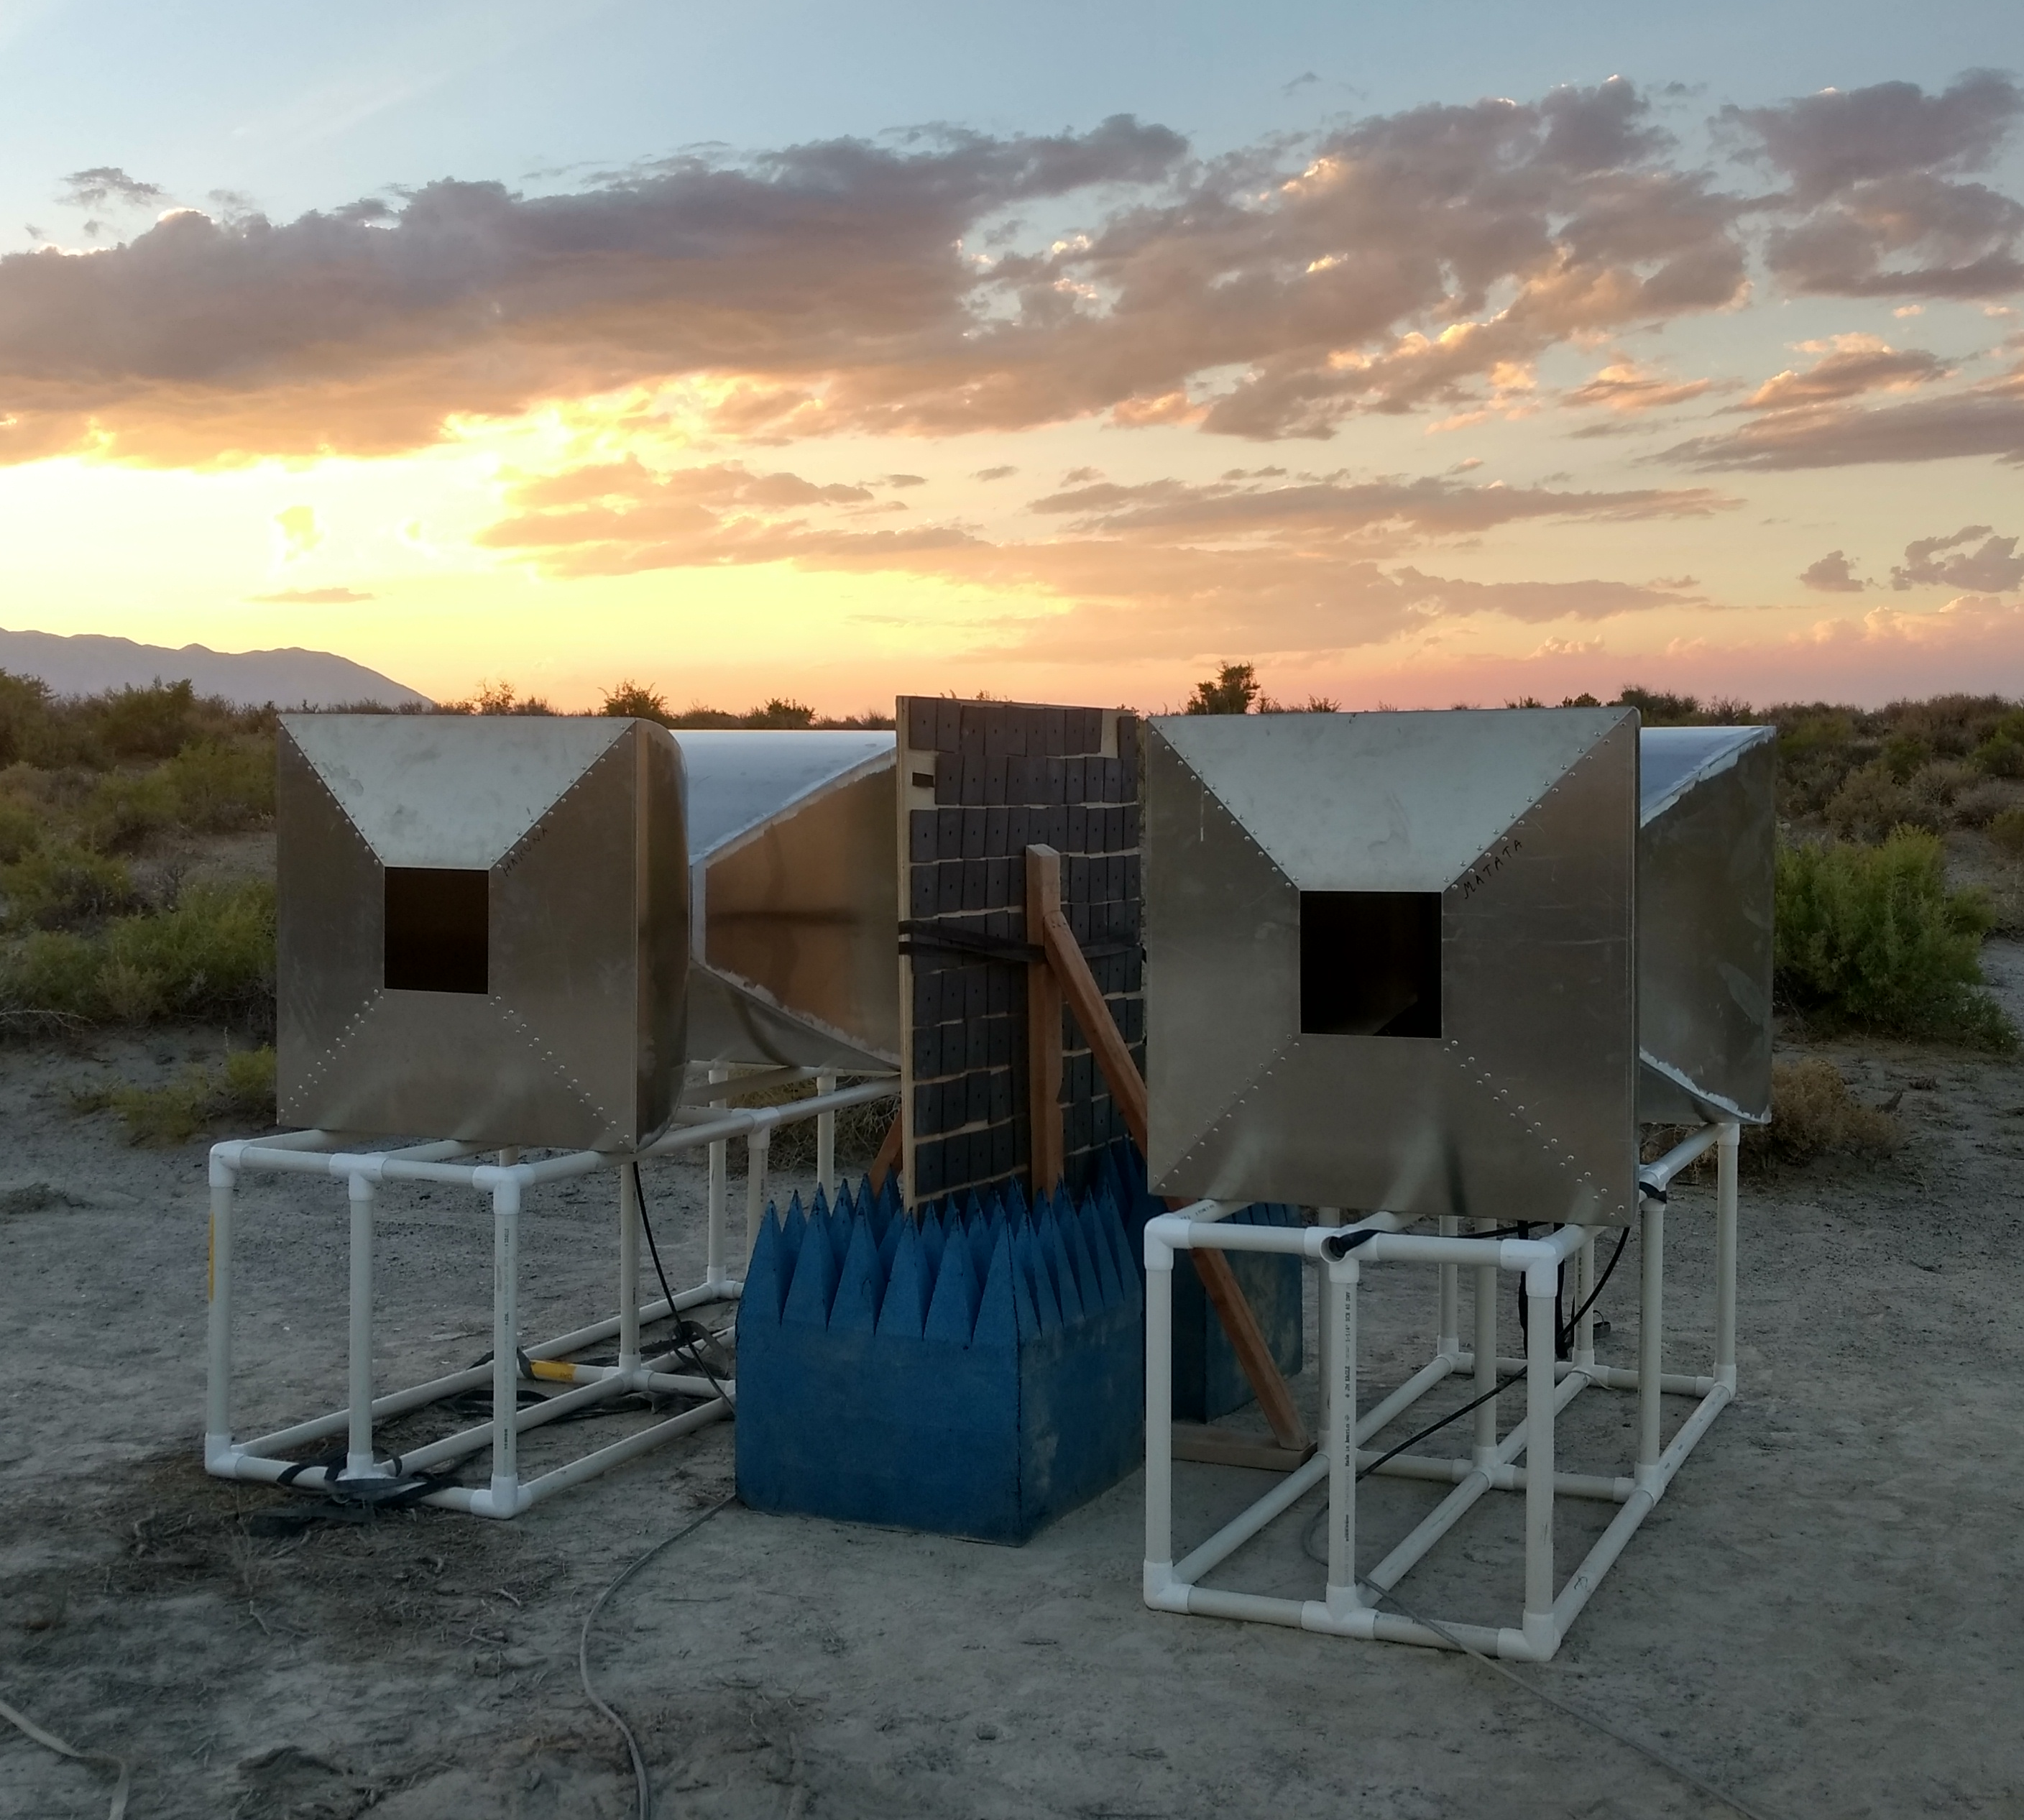
\includegraphics[width=\linewidth]{field-test.png}
    \end{center}
    \caption{
        Shown here is a simple diagnostic field set-up that could be used to 
        evaluate an absorber's ability to mitigate cross-talk between elements.  
        Here we used a densely-packed configuration of ferrite tiles that have 
        been propped up on some of our pyramidal foam absorber for additional 
        height.
    }
    \label{fig:field-test}
\end{figure}

Presently, we don't have any field results for how effective the absorptive 
walls are at mitigating cross-talk between antennas. The current iteration of 
the simulation assumes zero cross-talk between antennas, i.e. all sensitivity 
to the monopole comes from the presence of the dissipative absorber 
walls~\citep{venumadhav2016}.

We also haven't tested how the absorber behaves at the edges. Most importantly, 
we don't have a good grasp on how big of a problem diffraction over the top of 
the baffle walls is, and we don't have a model of the smoothing parameter $a$ 
from Eq.~\eqref{eq:absorber-baffle} or how it evolves with different baffle 
shapes. For the simulation, we have assumed that there is no diffraction and 
that the roll-off in absorber effectiveness is fairly sharp with $a = 0.01$.

ROLL-OFF IS FIRST ORDER APPROXIMATION OF DIFFRACTION, WE DON'T KNOW HOW EXACTLY 
TO PARAMETERIZE $a$, DISCUSS HOW DIFFERENT $a$ VALUES IMPACT GLOBAL SIGNAL 
RECOVERY

\subsection{Array Parameters}

Next, we must construct our model array. Basically, this means we must decide 
on the placement of our antenna-absorber elements. Our intuition tells us that 
the closer the elements are spaced to each other, the more sensitivity we will 
have to the monopole. But, of course, we don't yet know what the final baffle 
design for the elements is, and therefore we don't know how much space we will 
have to leave between elements.

At this level of the simulation, we are simply trying to determine what level 
of sensitivity we can expect across our full science frequency band at many 
different separations. We have chosen to test six possible separations: 1.5 m, 
3 m, 4.5 m, 6 m, 9 m, and 12 m. This corresponds to $\lambda/2$, $\lambda$, 
  $3\lambda/2$, $2\lambda$, $3\lambda$, and $4\lambda$ for a frequency of $\nu 
  = 100$ MHz, approximately the center of our science band.

\subsection{Modeling the Sky}

CITE HEALPIX, GORSKI

Finally, we need something to actually observe. We can construct a model of the 
sky using the AIPy Healpix tools, generating maps of the sky at multiple 
frequencies and storing them in bundles. These maps are contained and can be 
indexed by coordinates, making them easy to use for simulating observations and 
interferometric visibilities.

There are three things we hope to learn from our simulation, each one building 
upon the others.
\begin{enumerate}
 \item Can we observe a monopole sky using an interferometer?
 \item Can we see the reionization monopole in our interferometric observations 
  even with very bright foregrounds?
 \item Can we tease apart the monopole signal from the higher order, very 
  bright foreground terms?
\end{enumerate}

So fundamentally, we must be able to generate model skies for at least three 
cases: a monopole sky that models the frequency dependence and amplitude of the 
predicted reionization global signal, a monopole sky with a synchrotron 
frequency dependence, and a full global sky model for each frequency in our 
science band.

First off, we want to be able to model the monopole reionization signal. To do 
this, we will first generate a Healpix map filled with a flat brightness of 1 K 
for each frequency we want to simulate. We will then use the Accelerated 
Reionization Era Simulations (ARES) code developed by Jordan Mirocha to 
calculate the brightness temperature of the 21cm global signal at each 
frequency bin~\citep{mirocha2014}. Finally, we will scale the brightness of 
each map by the temperature calculated for its frequency, giving us a flat sky 
with an evolving brightness by frequency.

The same process can be used to generate a monopole synchrotron sky. In this 
case, the temperature at each frequency bin can be calculated via simple power 
law:

\begin{equation}
    \label{eq:synch-temp}
    T(\nu) = T(\nu_{150}) \Big(\frac{\nu}{\nu_{150}} \Big)^{-\beta}
\end{equation}

For our synchrotron sky, we have used the numbers presented 
in~\cite{rogers2008}, which lists a synchrotron sky brightness temperature of 
$T = 237$ K at $\nu = 150$ MHz and a scaling factor of $\beta = 2.5$. These 
numbers give us a galactic synchrotron brightness temperature of $T_{synch} = 
3700$ K at $\nu = 50 MHz$, which is the lowest frequency in our science band 
and therefore the brightest synchrotron bin. 

Finally, we want to be able to generate realistic sky maps with structure. We 
can do this using global sky models at multiple frequencies, such as those 
first presented in~\cite{haslam1982}.

\chapter{Sensitivity to the Monopole Sky}

\section{Simulated Visibilities}

Now all that remains is actually answering the question of whether or not this 
could work.  Can a traditional interferometer actually pick up a global sky 
signal?  And can we manipulate that sensitivity using the strategic placement 
of absorptive materials around our antennas?

Let's start by investigating the first question. Is an interferometer sensitive 
to the monopole sky? As described in Chapter~\ref{chap:logistics}, this can be 
be simulated, we just have to set our parameters appropriately.

We can begin with a very simplified proof-of-concept case. We will construct an 
array with no absorbers and a flat terrestrial horizon. Additionally, we will 
have beams with perfect receptivity in all directions, and a sky temperature of 
exactly $T_{sky} = 1.0$ K across our entire observational band. This will be 
our most basic unit test -- something with which to check our intuition against 
and prove that the idea behind HYPERION is sound.

As expected and  as can be easily seen in 
Figures~\ref{fig:flat-sky-no-abs-freq} and~\ref{fig:flat-sky-no-abs-uv}, all 
ground-based interferometers have a non-zero sensitivity to the monopole mode 
of the sky. Simlarly, we also find that the further we stray from the 
zero-spacing mode (i.e. as the number of wavelengths of separations increases), 
sensitivity to the monopole also quickly evaporates.

\begin{figure}
    \begin{center}
    \includegraphics[width=\linewidth]{/home/kara/documents/hyperion/memos/flat_sky_no_abs_freq.png}
    \end{center}
    \caption{
        Shown here is the absolute value of the visibility of a spectrally flat 
        monopole sky versus frequency. In this case, there are no absorptive 
        baffles, just the terrestrial horizon. As can be seen already, the 
        interferometer does have non-zero sensitivity to the monopole, though 
        it is plainly clear that the autocorrelation term (shown in blue) is 
        more sensitive than any of the non-zero interferometric baseline 
        pairings.
    }
    \label{fig:flat-sky-no-abs-freq}
\end{figure}

\begin{figure}
    \begin{center}
    \includegraphics[width=\linewidth]{/home/kara/documents/hyperion/memos/flat_sky_no_abs_uv.png}
    \end{center}
    \caption{
        REMAKE THIS FIGURE
        Shown here is the absolute value of the visibility of a spectrally flat 
        monopole sky with no absorber walls versus uv-baseline. As can be seen 
        already, the interferometer has a non-zero sensitivity to the monopole 
        at non-zero baseline separations.
    }
    \label{fig:flat-sky-no-abs-uv}
\end{figure}

But this simple unit test tells us much more than just the fact that HYPERION 
is feasible after all. We can also begin to see a characteristic shape of the 
sensitivity in the \emph{uv}-plane, with peaks and nulls placed at regular 
intervals in \emph{uv}-space. The predictability of this shape could allow us 
to use it as a calibration tool, if properly understood. In particular, it 
could be a valuable way to remove leakage from non-monopole terms into our 
signal. Given that this characteristic shape derives only from the monopole sky 
and the shape of the beam, we know that any observational deviations in this 
shape must come from the sky rather than the system. Therefore, it may be 
possible to use this information as a way to filter out non-monopole terms from 
the sky, thus ensuring that we won't mix up spectral wiggles from the 
combination of various non-monopole sky sources with our expected wiggly 
reionization global signal, as seen in Fig.~\ref{fig:global-signal}. Instead, 
we can, effectively, select just the monopole terms of the sky -- the galactic 
synchrotron background and the reionization global signal -- thus ensuring that 
the only terms we're left with have simple relationships with frequency that 
can be easily parsed from the frequency-independent evolution of the 
reionization term.

Additionally, this characteristic shape could enable  us to do some weighting 
of our observational data. By knowing exactly what modes we expect to see the 
monopole term at its brightest and dimmest, we could properly weight and 
interpret data at each mode and frequency, enabling us to better compare data 
points at different points in \emph{uv}-space and frequency.

So we have established that we can detect the monopole with an interferometer, 
which is step one. But, as we can see, that sensitivity is faint, especially at 
the high-frequency end of our science band. That by itself is not wholly 
problematic -- we could just run our observation longer and beat down our 
sensitivity, assuming we still keep our spacing close enough that our 
observations don't have to run infinitely long. What is problematic is the 
strong cross-talk between elements that we know we'll face when we place them 
that close. We need to make our elements invisible to each other, and we think 
we can simultaneously enhance our sensitivity to the monopole as well.

In our next set of tests, we include the absorptive baffles around each 
antenna, as described in previous chapters. Using the absorption profile of the 
ferrite tiles, as seen in Fig.~\ref{fig:fe-absorption}, we can see how the 
monopole sensitivity is changed in the presence of the baffles.

As can be seen in Figures~\ref{fig:flat-sky-fe-abs-freq} 
and~\ref{fig:flat-sky-fe-abs-uv}, the sensitivity of the autocorrelation signal 
drops off, which is a nice sanity check on this test -- less signal from the 
sky getting picked up by the antenna means less bright visibility on the other 
end. However, while the spectral shape of the interferometric sensitivity 
changes, we don't see the same drop in sensitivity in the cross-correlation 
terms that we do in the auto-correlation. Moreover, as seen in 
Fig.~\ref{fig:flat-sky-fe-abs-freq}, we actually see \emph{increased} 
sensitivity at the high-frequency end of our science band.

\begin{figure}
    \begin{center}
    \includegraphics[width=\linewidth]{/home/kara/documents/hyperion/memos/flat_sky_with_fe_abs_freq_01.png}
    \end{center}
    \caption{
        REWRITE CAPTION
        Shown here is the absolute value of the visibility of a spectrally flat 
        monopole sky versus frequency, for an array with absorptive baffles 
        constructed from ferrite tiles.
    }
    \label{fig:flat-sky-fe-abs-freq}
\end{figure}

Additionally, we can see in Fig.~\ref{fig:flat-sky-fe-abs-uv} that the 
baselines no longer completely line up their peaks and nulls in $uv$-space.  
This makes it slightly harder for us to calibrate, as we will have to compare 
the monopole measurements of each baseline only against matching baselines in 
the array, rather than by matching the measurements at each $uv$-coordinate in 
different baseline pairs. It would have been quite convenient for our 
calibration and data processing purposes to be able to sample points of pure 
non-monopole foreground at multiple frequencies. However, there are still nulls 
in multiple frequencies, they just only apply to one baseline at a time, making 
them less universally helpful for data weighting and analysis.

\begin{figure}
    \begin{center}
    \includegraphics[width=\linewidth]{/home/kara/documents/hyperion/memos/flat_sky_with_fe_abs_uv_01.png}
    \end{center}
    \caption{
        REWRITE CAPTION
        Shown here is the absolute value of the visibility of a spectrally flat 
        monopole sky with ferrite absorber walls versus uv-baseline.
    }
    \label{fig:flat-sky-fe-abs-uv}
\end{figure}

\section{Recovered Global Signal}

talk about how actual observations will be noisy (random noise from instrument, 
plus changing non-monopole sky), want to see if these characteristic spectral 
shapes that we see in our monopole simulation can be used to recover the 
monopole signal

show figures (need to be generated) from totalSensitivity script, show that we 
can observe monopole using noisy input data

next steps would be to accurately input non-monopole modes (using global sky 
model as one of the input maps, alongside 21cm hypothesized global signal) and 
see if reionization can still be detected

\chapter{Conclusion}

As we have shown, the ideas behind HYPERION are sound. We can manipulate our 
sensitivity to the global signal by imposing a step function onto the beam of 
our antennas -- thereby converting the monopole mode into a series of higher 
order modes with known scale coefficients. We can create this step function 
both by building HYPERION on the Earth and using the pre-existing horizon to 
our advantage, and by artificially raising that horizon by building absorptive 
walls around each antenna. Through in-lab testing, we have found that the most 
promising absorptive material at our low-frequency ranges is ferrite, though we 
are also interested in the idea of a resistive mesh, either on its own or 
layered with the ferrite, depending on its performance. Once we know about the 
final overall performance of an absorber across our science band, we can 
simulate a given array design's sensitivity to the monopole sky, and thereby 
generate the scale coefficients for each antenna pairing in the array. We can 
use these scale coefficients to the calibrate and process the observational 
data, recovering the monopole sky and finally getting a glimpse of the global 
signal.

These results are quite promising, particularly because, as seen in 
Fig.~\ref{fig:recovered-mismatched}, this data processing method is robust 
against at least some types of miscalibration. We were able to completely 
mismatch the true and simulated absorber profiles, and ended up recovering a 
global signal that was only approximately 5\% different from the true input 
signal. This indicates that, should HYPERION ever be constructed, those 
operating it need not worry about constantly monitoring the state of the 
absorber baffles to get a perfectly accurate measure of their absorptivity for 
each measurement made -- so long as we take care in our initial measurements of 
the absorber baffles, we can be confident that they will remain good enough to 
provide us excellent results in our observations.

Now that we know that these measurements are feasible, and possibly more robust 
to systemic error than our experimental predecessors, we must now continue to 
seek a better understanding of our instrumental design and how to optimize it 
in the face of real observational adversity. So far, we have taken the very 
optimistic view in our simulations that the sky is purely monopole, that there 
are no higher order modes in our signal. In reality, we know that the sky at 
these frequencies is full of galactic structure and extragalactic point 
sources. We simply don't know how well this method of data analysis will work 
when we have a realistically spatially-polluted sky.

The next step to prove the merit of a monopole interferometer would be to input 
a complex sky into the model and see how it behaves. Using accurate global sky 
models alongside our theoretical reionization signal, we can perform the same 
process described in Section~\ref{sec:recovered-signal} and assess our ability 
to recover the reionization global sky, and develop new tools as necessary.

We must also further investigate the realities of the absorbers and how best to 
construct them. To start, we may first assess the viability of the resistive 
mesh concept, testing its absorption across our frequency band and comparing it 
to that of the ferrite tiles. Next, we must begin to explore the full 
electromagnetic system of our antenna-absorber pairs. How does diffraction 
affect our absorber spatial profile? Is there coupling between the absorber and 
the antenna? If so, how does that change our results?

The answers to these questions will determine the long-term viability of this 
method. At present, all we know is that the idea behind a monopole 
interferometer is far less far-fetched than it may have originally seemed. With 
proper calibration and experimental design, it very well could serve a key 
place in the search for understanding of the epoch of reionization.


\appendix
\chapter{The Flat-Sky Approximation and Its Limitations}
\label{appendix}

In Eq.~\eqref{eq:van-cittert}, we made one implicit assumption -- that we are 
working in only two dimensions. This, of course, is not true. 

In reality, if one is hoping to utilize the convenient Fourier nature of the 
brightness and visibility planes, the van Cittert-Zernicke theorem should be 
written in terms of \emph{(u,v,w)} coordinates, rather than just \emph{(u,v)}.  
The full (idealized) measurement equation can thus be written as:

\begin{equation}
    V(u,v,w) = \iint I(l,m) e^{-2\pi i (ul + vm + w\sqrt{1 - l^2 - m^2})} dl dm
    \label{eq:full-measurement}
\end{equation}

The next step is to assume that $l$ and $m$ are small, such that $\sqrt{1 - l^2 
- m^2} \approx 1$, allowing the $e^{-2\pi i w}$ term to be removed from the 
integral by applying the proper phasing to the measured visibility and the 
measurement equation to be simplified to a 2D Fourier transform sampled in the 
\emph{uv}-plane. This procedure is called the \emph{flat-sky approximation}.

This approximation works well for many applications in astronomy, particularly 
in the observation of point sources or small extended sources in the sky (up to 
about $\pm10^\circ$ or so, where $l \equiv \sin\theta \approx \theta$).  
However, as the observed area in the sky gets larger, it becomes impossible to 
apply an absolutely correct phasor to the 2D integral, and the $w$-term instead 
introduces a spatially varying departure from the 2D Fourier transform the 
further from the phase center you are.

So, obviously, in the case where you're trying to use an interferometer to 
observe a global phenomenon (such as the reionization global signal), the flat 
sky approximation simply won't do. In the case that one is attempting to 
perform sky imaging, then care must be taken to navigate the pitfalls of the 
flat-sky approximation, including the use of clunky or expensive algorithms 
such as W-projection. In our case, we are not trying to image the sky at all, 
rather we're just attempting to understand the distribution of power in the 
visibility domain. We can therefore avoid the $(u,v)$ to $(l,m)$ confusion 
entirely and calculate our visibilities directly based on our knowledge of the 
source direction $\mathbf{s}$ and the baseline separation $\mathbf{b}$.


\bibliography{references}{}
\bibliographystyle{apj}

%\printbibliography

\end{document}
